% !TeX root = ./0-Tesis-de-maestria-JLBG.tex
\label{cap: introduccion}

Desde mediados del siglo pasado, se han propuesto diversas técnicas para manipular objetos en la escala micro y nanométrica \cite{ashkin1970acceleration, ashkin1987optical, Ashkin, custance2009atomic, dholakia2011shaping, marago2013optical, romo2020controlled}. Las pinzas ópticas, basadas en las fuerzas electromagnéticas producidos por haces de luz enfocados, han sido ampliamente utilizadas para atrapar y mover microobjetos, incluyendo virus y bacterias, lo que ha tenido un gran impacto en el desarrollo tecnológico y médico \cite{ashkin1970acceleration, ashkin1987optical, Ashkin}.  

En 2004, Javier García de Abajo publicó un trabajo sobre la posibilidad de manipular nanoobjetos mediante microscopios electrónicos de transmisión (TEMs por sus siglas en inglés) \cite{GarciadeAbajo0}. Desde entonces, se ha demostrado experimentalmente que los TEM pueden usarse para inducir movimiento y rotación en nanopartículas (NPs) \cite{Batson01, zheng2012electron}, lo que ha llevado al desarrollo de una técnica de manipulación llamada <<pinzas electrónicas>> \cite{Batson, oleshko2005electron, Oleshko}.

En diversos estudios experimentales sobre pinzas electrónicas, se ha observado que la transferencia de momento angular y lineal del haz de electrones a la NP depende tanto de la velocidad del haz de electrones como del parámetro de impacto, que es la distancia efectiva entre la trayectoria del haz de electrones y el centro de la NP \cite{OLESHKO2013203, Oleshko, Batson, Batson01, zheng2012electron, xu2010transmission}.  Al modificar el parámetro de impacto, se puede inducir una interacción atractiva o repulsiva entre el haz de electrones y la NP, y también es posible modificar la dirección del giro inducido sobre la NP \cite{OLESHKO2013203, Batson, Oleshko}. 

El microscopio electrónico de transmisión de barrido (STEM por sus siglas en inglés) forma imágenes mediante haces enfocados de electrones que barren el área de interés, utilizando los electrones esparcidos por la muestra \cite{Batson}. En la Fig. \ref{fig: Batson STEM} se muestra un par de NPs de oro, una grande y una pequeña, siendo escaneada por el haz de un STEM, dentro de la región con contorno blanco. Durante el barrido, el haz de electrones permanece detenido el 20\% del tiempo al inicio de cada una de las líneas a escanear, lo que produce una corriente neta de electrones que viajan fuera de la NP. Esta corriente se ilustra como una región sombreada en azul en la Fig. \ref{fig: Batson STEM}. Por lo tanto, aunque el haz de electrones barre toda la muestra que se observa en el STEM, hay un parámetro de impacto efectivo respecto a la superficie de la NP.

\begin{figure}[h!]
\centering
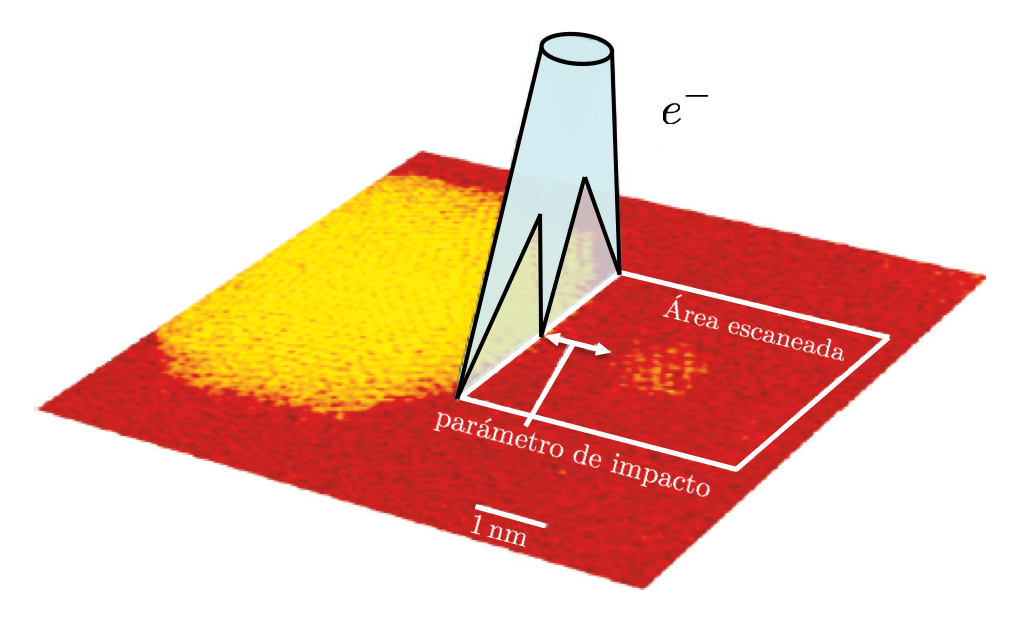
\includegraphics[width=0.6\linewidth]{17-imagenes/1-Intro/STEM}
\caption{\label{fig: Batson STEM} Esquema de la interacción dentro de un STEM, entre un haz de electrones con un par de nanopartículas de oro, reproducido y adaptado de la Ref \cite{Batson}.} 
\end{figure}

En la Fig. \ref{fig: Batson momentum transfer}, se presentan algunos de los resultados reportados en la Ref. \cite{Batson}, que muestran seis imágenes de STEM de una NP de oro de $1.5$ nm en presencia de otra de $5$ nm, a diferentes tiempos. En todas las imágenes de la Fig. \ref{fig: Batson momentum transfer}, el parámetro de impacto efectivo se encuentra a la izquierda de la NP (cerca del borde izquierdo de la imagen). Las tres imágenes superiores de la Fig. \ref{fig: Batson momentum transfer}, tomadas con un parámetro de impacto efectivo de $4.5$ nm, muestran una interacción atractiva entre el haz y la NP, ya que se puede observar que la NP se acerca al borde izquierdo de las imágenes, atravesando la línea punteada blanca colocada como ayuda visual. Por el contrario, en las imágenes inferiores de la Fig. \ref{fig: Batson momentum transfer}, cuyo  parámetro de impacto efectivo es de $1$ nm,  se observa que la NP se aleja del haz, atravesando la línea punteada blanca en dirección opuesta y acercándose al borde derecho de la imagen, lo que indica una interacción repulsiva. Utilizando las líneas guía que se han trazado en las facetas de la NP grande, que forman un polígono, se puede apreciar que en las tres imágenes superiores la NP gira en sentido horario, mientras que en las inferiores, al cambiar el parámetro de impacto, gira en sentido antihorario.

\begin{figure}[h!]
\centering
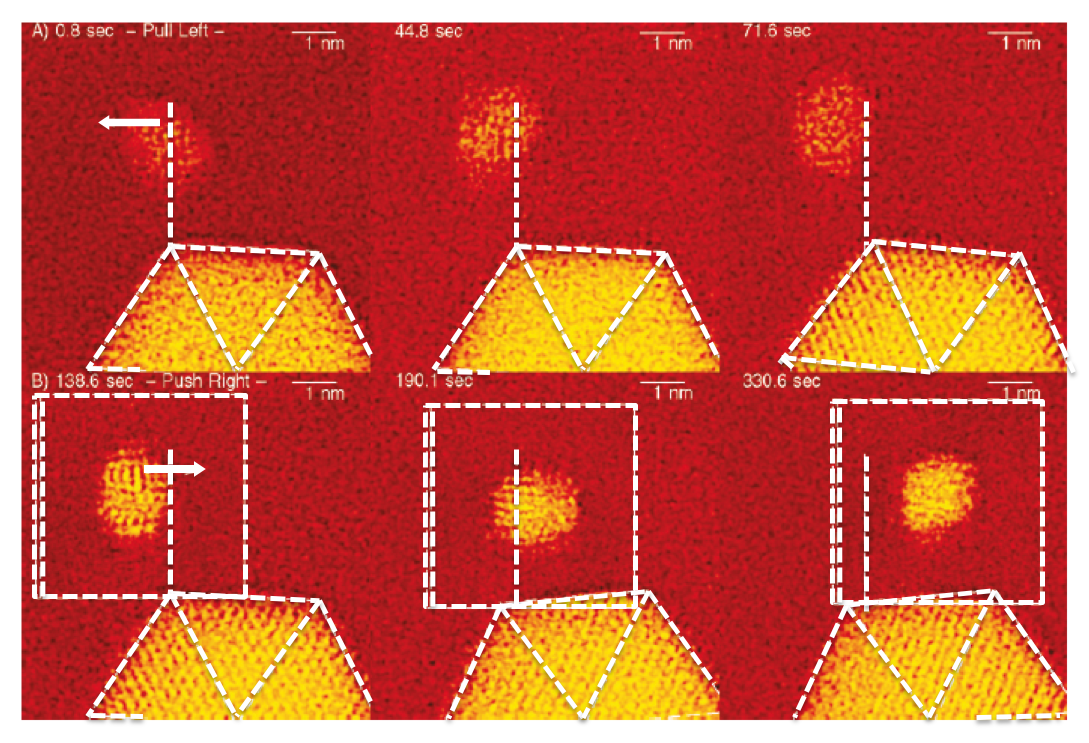
\includegraphics[width=0.6\linewidth]{17-imagenes/1-Intro/Batson}
\caption{\label{fig: Batson momentum transfer} Resultados reproducidos y adaptados de la Ref. \cite{Batson}, donde se observa transferencia de momento angular y lineal de un haz de electrones STEM a nanopartículas de oro, suspendidas en un sustrato de carbono.} 
\end{figure}

Para desarrollar la técnica de pinzas electrónicas, es necesario un entendimiento teórico del problema. Los haces electrónicos en un STEM pueden alcanzar $400$ keV de energía cinética, con una corriente eléctrica del orden de pA, lo que equivale a un pulso de electrones rápidos viajando a velocidad constande alcanzando velocidades de hasta $v=0.83 c$ (donde $c$ es la velocidad de la luz). De lo anterior, se deduce que el tiempo de emisión de cada electrón es de $10^{-8}$ s. Como la vida media de las excitaciones dentro de un metal es de $\sim 10^{-14}$ \cite{quijada2010lifetime}, se puede asumir que la NP interactúa con un electrón a la vez \cite{de1999relativistic, GarciadeAbajo-1, deabajo2021optical}. Además,  los haces de electrones en estudios de STEM se desvían a ángulos del orden de miliradianes \cite{deabajo2021optical, Rivacoba1, krehl2018spectral}, por lo que se puede considerar que se mueven en línea recta, siempre y cuando los electrones viajen fuera de la NP. Por lo anterior, se puede modelar la trayectoria del electrón rápido como $\vv{r}(t)=(b, 0, vt)$, donde $v$ es la velocidad del electrón y $b$ es la distancia entre el centro de la NP y la trayectoria del electrón, denominada como parámetro de impacto, como se muestra en la Fig. \ref{fig: system mine}. La respuesta electromagnética de la NP, se puede modelar mediante su función dieléctrica $\epsilon(\w)$.

\begin{figure}[ht!]
\centering
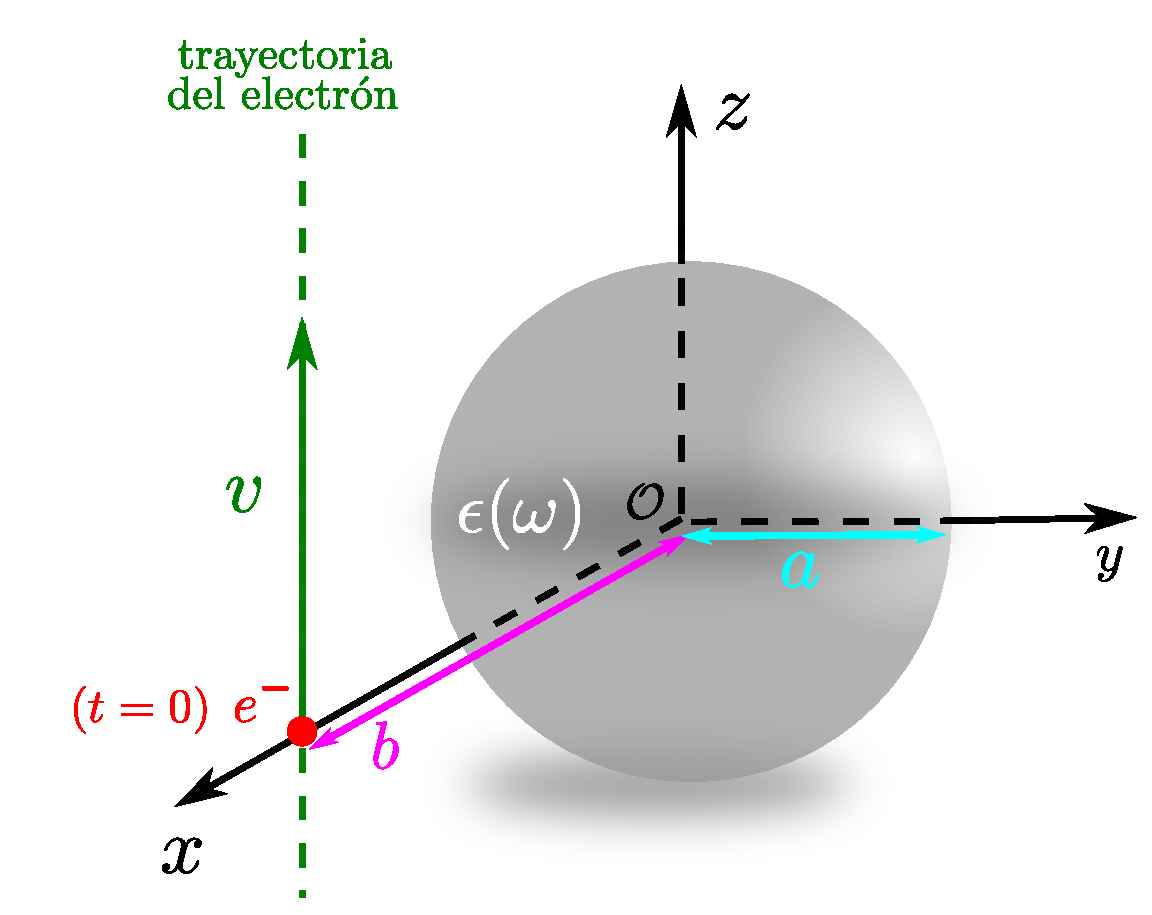
\includegraphics[width=0.5\linewidth]{17-imagenes/1-Intro/system_NP.pdf} 
\caption{Nanopartícula de radio $a$, centrada en el origen de coordenadas, modelada mediante una función dieléctrica $\epsilon(\w)$ en vacío. La trayectoria del electrón (punto marrón), con parámetro de impacto $b$ y viajando a velocidad constante $v$, se muestra como una línea punteada de color verde. \label{fig: system mine}}
\end{figure}

La interacción entre haces de electrones y NPs esféricas ha sido abordado desde la perspectiva de la electrodinámica clásica \cite{GarciadeAbajo0, PRBCoronado, Lagos2, Batson2, xu2010transmission}. Los trabajos citados anteriormente se han centrado en el cálculo de transferencia de momento lineal mediante la solución de las ecuaciones de Maxwell en el espacio de frecuencias. Para ello, se ha utilizado una expansión multipolar que permite separar la contribución eléctrica y magnética de la interacción, así como la contribución de cada orden multipolar. Sin embargo, es necesario tener precaución al elegir la función dieléctrica para modelar la respuesta de las NPs. Dado que experimentalmente se mide la función dieléctrica en un rango finito de frecuencias, es necesario extrapolarla e interpolarla para realizar la integral del tensor de esfuerzos de Maxwell en todo el espacio de frecuencias. Si no se tiene cuidado suficiente, este proceso puede dar como resultado una función dieléctrica no causal, que no satisface las relaciones de Kramers-Kronig. A pesar de que los trabajos citados en las Refs. \cite{GarciadeAbajo0, PRBCoronado, Lagos2, Batson2, xu2010transmission} han logrado reproducir el comportamiento atractivo y repulsivo de la interacción, estudios recientes han mostrado que dichos trabajos obtuvieron resultados no físicos al modelar la respuesta electromagnética de la NP mediante funciones dieléctricas no causales \cite{castrejon2021effects, castrejon2021phdthesis}. En estos trabajos, se muestra que si se elimina el comportamiento no causal de las funciones dieléctricas, no aparece la interacción repulsiva reportada experimentalmente. En la Ref. \cite{castrejon2021phdthesis} se resuelve de forma semi-analítica las integrales en el espacio de frecuencia, que previamente se resolvían de forma numérica en las Refs. \cite{GarciadeAbajo0, PRBCoronado, Lagos2, Batson2, xu2010transmission}. Lo anterior permite conocer de manera exacta la contribución en el espacio de frecuencias de cada multipolo, eléctrico o magnético, a la transferencia de momento lineal, logrando así calcular la transferencia de momento lineal de electrones rápidos a NPs grandes (de hasta $a=50$ nm de radio).


%A pesar de lo anterior, un estudio detallado de la dinámica angular es necesario para el desarrollo de la técnica de pinzas electrónicas. Recientemente se han publicado estudios de la TMA de electrones rápidos a NPs pequeñas, de hasta $a=5$ nm de radio \cite{castellanos2021phdthesis, castellanos2021angular,castellanos2023theory}, donde se usan dos métodos para calcular la TMA.

La técnica de pinzas electrónicas también requiere un estudio detallado de la transferencia de momento angular (TMA). En trabajos previos se ha discutido la dinámica angular de forma somera (ver por ejemplo la Ref. \cite{GarciadeAbajo-1}), pero estudios recientes han permitido calcularla en NPs pequeñas de hasta $a=5$ nm de radio utilizando dos métodos distintos. El primer método modela la respuesta electromagnética de la NP como un dipolo puntual $\vv{p}$, mediante el tensor de polarizabilidad, lo que es válido únicamente para NPs pequeñas \cite{castellanos2021angular}. El segundo método resuelve numéricamente las integrales de superficie del tensor de esfuerzos de Maxwell\cite{castellanos2023theory, castellanos2021phdthesis} en el espacio de frecuencias. Sin embargo, el cálculo numérico limita el tamaño de las NPs que se pueden estudiar (menores a 5 nm), debido al tiempo de cómputo necesario, como se ha reportado en las Refs. \cite{castellanos2021phdthesis, castellanos2021angular,castellanos2023theory}. Por lo tanto, los métodos mencionados solo permiten el cálculo de la TMA en nanopartículas pequeñas, de hasta $a=5$ nm de radio.

Se ha demostrado que existen términos en el tensor de esfuerzos de Maxwell que corresponden a los campos externos producidos por el electrón y que no contribuyen a la TMA total. Por lo tanto, se ha demostrado que la integral del tensor de esfuerzos de Maxwell que contiene solo a los campos electromagnéticos del electrón debe anularse. Además, se ha demostrado que el término de interacción en el tensor de esfuerzos, que incluye tanto a los campos electromagnéticos del electrón como a los campos esparcidos por la nanopartícula, es el que más contribuye a la transferencia de momento, y que el término que incluye únicamente los campos esparcidos por la nanopartícula, aunque es pequeño, no se anula \cite{castellanos2021phdthesis, castrejon2021phdthesis}.

En este trabajo se presenta un estudio teórico de la TMA de electrones rápidos a NPs, utilizando un enfoque de electrodinámica clásica. En el capítulo \hyperref[cap: teoria metodos]{Capítulo} \ref{cap: teoria metodos} se desarrollan la teoría y métodos necesarios para discutir la deducción de los campo electromagnéticos producidos por un electrón relativista en movimiento rectilíneo uniforme, así como los campos electromagnéticos esparcidos por una NP centrada en el origen cuya respuesta electromagnética se modela mediante su función dieléctrica $\epsilon(\omega)$. Además, se enuncia el teorema de conservación de momento angular en electrodinámica y, a partir de ello, se calcula en general la TMA del electrón rápido a la NP mediante una integral del tensor de esfuerzos de Maxwell en el espacio de frecuencias. En el \hyperref[cap: resultados]{Capítulo} \ref{cap: resultados} se presentan los resultados de esta tesis de maestría, donde se calcula una solución semi-analítica de la integral del tensor de esfuerzos de Maxwell en el espacio de frecuencias que permite calcular de forma eficiente la TMA. Finalmente, en la sección de \hyperref[conclusiones]{Conclusiones}, se resumen los resultados más relevantes y sus implicaciones, así como las posibles vías para futuras investigaciones que se derivan de los resultados publicados en esta tesis.
